\chapter{Arhitektura i dizajn sustava}
		
		%\textbf{\textit{dio 1. revizije}}\\

		%\textit{ Potrebno je opisati stil arhitekture te identificirati: podsustave, preslikavanje na radnu platformu, spremišta podataka, mrežne protokole, globalni upravljački tok i sklopovsko-programske zahtjeve. Po točkama razraditi i popratiti odgovarajućim skicama:}
	%\begin{itemize}
		%\item 	\textit{izbor arhitekture temeljem principa oblikovanja pokazanih na predavanjima (objasniti zašto ste baš odabrali takvu arhitekturu)}
		%\item 	\textit{organizaciju sustava s najviše razine apstrakcije (npr. klijent-poslužitelj, baza podataka, datotečni sustav, grafičko sučelje)}
		%\item 	\textit{organizaciju aplikacije (npr. slojevi frontend i backend, MVC arhitektura) }		
	%\end{itemize}

	
		Arhitektura sustava oblikovana je tako da se sastoji od tri podsustava:
		
		\begin{itemize}
			\item Web preglednik
			\item Web poslužitelj
			\item Baza podataka
		\end{itemize}
		
		\textbf{Web preglednik} služi korisniku za pristup poslužitelju i podacima u bazi podataka. To je program kojim korisnik može slati zahtjeve do poslužitelja za neku uslugu, u obliku dohvaćanja ili slanja podataka do poslužitelja. Web poslužitelj će nakon primitka zahtjeva od korisnika kroz Web preglednik prikazati odgovor na zahtjev. Dakle, Web preglednik je prvi korak za krajnjeg korisnika u interakciji sa sustavom u cjelini.
		
		
		\textbf{Web poslužitelj} je središnja komponenta sustava gdje se događaju svi važni izračuni te strukturiranje odgovora korisniku, a isto tako i pristup bazi podataka. To je program na jednom ili više računala, odnosno poslužitelja, koji interagira s jednim ili više korisnika. Zahtjeve prima preko HTTP protokola te vraća odgovor u obliku HTML dokumenta koji se prikazuje korisniku u njegovom Web pregledniku, potrebne podatke pohranjuje i ažurira u bazi podataka.
		
		
		\textbf{Baza podataka} je podsustav koji služi za pohranu svih potrebnih podataka. Backend strana Web aplikacije pristupa joj te upravlja podacima. Zbog učestalosti pristupa podacima u bazi podataka, od velike je važnosti da ona radi brzo i efikasno te je stoga bitno bazu podataka oblikovati efikasno i normalizirano.\\
		
		Arhitekturni stil koji je odabran za izradu sustava je model-pogled-nadglednik (engl. Model-View-Controller ili kraće MVC). MVC, ujedno i oblikovni obrazac, karakterizira njegova tri sloja model, view i controller.  
		
		\begin{itemize}
			\item \textbf{Model} je glavna komponenta ovog arhitekturnog stila. Sadrži razrede koji su vrlo slični tablicama u bazi podataka. Razredi modela opisuju strukture podataka te sadrže pravila i logiku rada aplikacije.
			\item \textbf{View} je komponenta koja se jedina ne nalazi na poslužiteljskoj strani. Ona služi za interakciju sustava s korisnikom, kako kroz zahtjeve korisnika, tako i kroz reprezentaciju odgovora poslužitelja krajnjem korisniku.
			\item \textbf{Controller} je komponenta koja upravlja zahtjevima krajnjeg korisnika na temelju modela. Također, ova komponenta upravlja odgovorima koji se dalje šalju do komponente View.
		\end{itemize}
		
		
		U izgradnji sustava koristi se objektno orijentirana paradigma. Za ovaj sustav to je programski jezik Java te radni okvir Spring koji je korišten za izradu backenda. Za izradu frontend dijela sustava, odnosno Web aplikacije upotrebljava se programski jezik JavaScript te biblioteka React. Uz to, za vanjsku komunikaciju kao pomoć u radu aplikacije, koristi se vanjski rječnik uz pomoć aplikacijskog sučelja.\\
		
		\newpage

				
		\section{Baza podataka}
			
			%\textbf{\textit{dio 1. revizije}}\\
			
		%\textit{Potrebno je opisati koju vrstu i implementaciju baze podataka ste odabrali, glavne komponente od kojih se sastoji i slično.}
		
\hspace*{6mm} Za potrebe rada sustava kojeg gradimo koristit ćemo relacijsku bazu podataka čiji su glavni elementi relacije. Relacije možemo promatrati kao tablice definirane svojim imenom te atributima. Relacijski model nastao je na temelju ER modela baze podataka čiji su temeljni elementi entiteti i veze. Zadatak baze podataka je brzo, kompaktno te jednostavno pohranjivanje, izmjenu te uklanjanje raznih podataka. Za ovaj sustav, to su podaci o korisničkim računima, podaci o pohranjenim rječnicima te riječima u njima, opisi riječi te stadij učenja u kojem se nalazi korisnik sustava. U skladu s tim, definiramo bazu podataka sastavljenu od entiteta:
			
			\begin{packed_item}
				
				\item Account
				\item AccountType
				\item CurrentState
				\item Pot
				\item LearningMode
				\item Dictionary
				\item Language
				\item Phrase
				\item Word
				\item wordInDict
				\item wordInPot
				
			\end{packed_item}
		
			\subsection{Opis tablica}
			

%				\textit{Svaku tablicu je potrebno opisati po zadanom predlošku. Lijevo se nalazi točno ime varijable u bazi podataka, u sredini se nalazi tip podataka, a desno se nalazi opis varijable. Svjetlozelenom bojom označite primarni ključ. Svjetlo plavom označite strani ključ}
				
				
				\hspace*{6mm} \textbf{Account} Ovaj entitet sadrži informacije o korisničkom računu. Njegovi atributi su: accountID, accountEmail, personName, personSurname, accountPassword te accountTypeID. Ovaj entitet u vezi \textit{Many-to-One} je s entitetom AccountType preko atributa accountTypeID, u vezi \textit{One-to-Many} s entitetom Pot preko atributa accountID te u vezi \textit{One-to-Many} s entitetom CurrentState preko atributa accountID.
				
				\begin{longtblr}[
					label=racun,
					entry=none
					]{
						width = \textwidth,
						colspec={|X[8,l]|X[6, l]|X[18, l]|}, 
						rowhead = 1,
					} %definicija širine tablice, širine stupaca, poravnanje i broja redaka naslova tablice
					\hline \SetCell[c=3]{c}{\textbf{Account}}	 \\ \hline[3pt]
					\SetCell{LightGreen}accountID & INT	&  	Jedinstven identifikator korisnika generiran od strane baze podataka (surogatni ključ)  	\\ \hline
					accountEmail	& VARCHAR &   Jedinstvena adresa elektroničke pošte (alternativni ključ)	\\ \hline 
					personName & VARCHAR & Ime korisnika  \\ \hline 
					personSurname & VARCHAR	&  	Prezime korisnika	\\ \hline 
					accountPassword & VARCHAR & Kriptirana lozinka korisnika  \\ \hline
					\SetCell{LightBlue} accountTypeID	& INT &   Identifikator vrste računa korisnika	\\ \hline 
				\end{longtblr}
				
				\textbf{AccountType} Ovaj entitet sadrži informacije o vrsti korisničkog računa (radi li se o učeniku ili administratoru riječi). Njegovi atributi su: accountTypeID te accountTypeName. Ovaj entitet u vezi \textit{One-to-Many} je s entitetom Account preko atributa accountTypeID.
				
				\begin{longtblr}[
					label=vrstaRacuna,
					entry=none
					]{
						width = \textwidth,
						colspec={|X[8,l]|X[6, l]|X[18, l]|}, 
						rowhead = 1,
					} %definicija širine tablice, širine stupaca, poravnanje i broja redaka naslova tablice
					\hline \SetCell[c=3]{c}{\textbf{AccountType}}	 \\ \hline[3pt]
					\SetCell{LightGreen}accountTypeID & INT	&  Jedinstven identifikator vrste računa generiran od strane baze podataka (surogatni ključ)  	\\ \hline
					accountTypeName	& VARCHAR &   Ime vrste računa	\\ \hline  
				\end{longtblr}
				
				\textbf{CurrentState} Ovaj slabi entitet sadrži informacije o trenutnom stanju u kojem se nalazi korisnik sustava. Njegovi atributi su: dictionaryID, accountID, learningModeID. Ovaj entitet u vezi \textit{Many-to-One} je s entitetom Dictionary preko atributa dictionaryID, u vezi \textit{Many-to-One} je s entitetom Account preko atributa accountID, u vezi \textit{Many-to-One} je s entitetom LearningMode preko atributa learningModeID.
				
				\begin{longtblr}[
					label=trenutnoStanje,
					entry=none
					]{
						width = \textwidth,
						colspec={|X[8,l]|X[6, l]|X[18, l]|}, 
						rowhead = 1,
					} %definicija širine tablice, širine stupaca, poravnanje i broja redaka naslova tablice
					\hline \SetCell[c=3]{c}{\textbf{CurrentState}}	 \\ \hline[3pt]
					\SetCell{LightGreen}dictionaryID & INT	&  	Jedinstven identifikator rječnika (strani ključ)	\\ \hline
					\SetCell{LightGreen}accountID & INT	&  	Jedinstven identifikator računa (strani ključ)	\\ \hline
					\SetCell{LightGreen}learningModeID & INT	&  	Jedinstven identifikator moda (strani ključ) učenja 	\\ \hline
				\end{longtblr}
				
				\textbf{Pot} Ovaj slabi entitet sadrži informacije o pojedinoj posudi riječi pridruženoj nekom korisniku. Njegovi atributi su: potID, accountID, expirationTime, potNumber. Ovaj entitet u vezi \textit{Many-to-One} je s entitetom Account preko atributa accountID, u vezi \textit{Many-to-Many} je s entitetom Word preko atributa wordID, potID, accountID.
				
				\begin{longtblr}[
					label=posuda,
					entry=none
					]{
						width = \textwidth,
						colspec={|X[7,l]|X[6, l]|X[19, l]|}, 
						rowhead = 1,
					} %definicija širine tablice, širine stupaca, poravnanje i broja redaka naslova tablice
					\hline \SetCell[c=3]{c}{\textbf{Pot}}	 \\ \hline[3pt]
					\SetCell{LightGreen}potID & INT	&  Jedinstveni identifikator posude riječi 	\\ \hline
					\SetCell{LightGreen}accountID & INT & Jedinstveni identifikator računa korisnika (strani ključ) \\ \hline
					expirationTime & INTERVAL & Vrijeme koje je potrebno proći kako bi se riječi iz posude pojavile u pitanju korisniku  \\ \hline 
					potNumber & INT	&  	Redni broj posude (alternativni ključ)	\\ \hline 
				\end{longtblr}
				
				\textbf{LearningMode} Ovaj entitet sadrži informacije o modu učenja u kojem je korisnik. Njegovi atributi su: learningModeID, learningModeDescription. Ovaj entitet u vezi \textit{One-to-Many} je s entitetom CurrentState preko atributa learningModeID. \newpage
				
				\begin{longtblr}[
					label=modUcenja,
					entry=none
					]{
						width = \textwidth,
						colspec={|X[11,l]|X[6, l]|X[15, l]|}, 
						rowhead = 1,
					} %definicija širine tablice, širine stupaca, poravnanje i broja redaka naslova tablice
					\hline \SetCell[c=3]{c}{\textbf{LearningMode}}	 \\ \hline[3pt]
					\SetCell{LightGreen}learningModeID & INT	&  Jedinstven identifikator moda učenja generiran od strane baze podataka (surogatni ključ)  	\\ \hline
					learningModeDescription	& VARCHAR &   Kratki opis moda učenja	\\ \hline 
				\end{longtblr}
				
				\textbf{Dictionary} Ovaj entitet sadrži informacije o rječniku za neki jezik. Njegovi atributi su: dictionaryID, dictionaryName, languageID. Ovaj entitet u vezi \textit{One-to-Many} je s entitetom CurrentState preko atributa dictionaryID, u vezi \textit{Many-to-One} s entitetom Language preko atributa languageID te u vezi \textit{Many-to-Many} s entitetom Word preko atributa dictionaryID, wordID.
				
				\begin{longtblr}[
					label=rjecnik,
					entry=none
					]{
						width = \textwidth,
						colspec={|X[7,l]|X[6, l]|X[19, l]|}, 
						rowhead = 1,
					} %definicija širine tablice, širine stupaca, poravnanje i broja redaka naslova tablice
					\hline \SetCell[c=3]{c}{\textbf{Dictionary}}	 \\ \hline[3pt]
					\SetCell{LightGreen}dictionaryID & INT	&  	Jedinstveni identifikator rječnika generiran od strane baze podataka (surogatni ključ)  	\\ \hline
					dictionaryName	& VARCHAR &   Ime rječnika	\\ \hline 
					\SetCell{LightBlue}languageID	& INT &   Jedinstveni identifikator jezika kojem je rječnik pridružen	\\ \hline 
				\end{longtblr}
				
				\textbf{Language} Ovaj entitet sadrži informacije o jeziku kojeg podržava sustav. Njegovi atributi su: languageID, languageCode, languageName. Ovaj entitet u vezi \textit{One-to-Many} je s entitetom Dictionary preko atributa languageID.
				
				\begin{longtblr}[
					label=jezik,
					entry=none
					]{
						width = \textwidth,
						colspec={|X[6,l]|X[6, l]|X[20, l]|}, 
						rowhead = 1,
					} %definicija širine tablice, širine stupaca, poravnanje i broja redaka naslova tablice
					\hline \SetCell[c=3]{c}{\textbf{Language}}	 \\ \hline[3pt]
					\SetCell{LightGreen}languageID & INT	&  Jedinstveni identifikator jezika generiran od strane baze podataka (surogatni ključ)	\\ \hline
					languageCode	& CHAR &   Troslovna kratica jezika	\\ \hline 
					languageName & VARCHAR & Ime jezika  \\ \hline 
				\end{longtblr}
				
				\textbf{Phrase} Ovaj entitet sadrži informacije o frazi koja bolje opisuje neku riječ. Njegovi atributi su: phraseID, phraseContent, wordID. Ovaj entitet u vezi \textit{Many-to-One} je s entitetom Word preko atributa wordID.
				
				\begin{longtblr}[
					label=fraza,
					entry=none
					]{
						width = \textwidth,
						colspec={|X[6,l]|X[6, l]|X[20, l]|}, 
						rowhead = 1,
					} %definicija širine tablice, širine stupaca, poravnanje i broja redaka naslova tablice
					\hline \SetCell[c=3]{c}{\textbf{Phrase}}	 \\ \hline[3pt]
					\SetCell{LightGreen}phraseID & INT	&  	Jedinstveni identifikator fraze generiran od strane baze podataka (surogatni ključ)  	\\ \hline
					phraseContent	& VARCHAR &   Tekst fraze	\\ \hline 
					\SetCell{LightBlue}wordID	& INT &   Jedinstveni identifikator riječi kojoj je fraza pridružena	\\ \hline 
				\end{longtblr}
				
				\textbf{Word} Ovaj entitet sadrži informacije o riječi koja je dodana u sustav. Njegovi atributi su: wordID, wordContent, wordPronunciation. Ovaj entitet u vezi \textit{Many-to-Many} je s entitetom Pot preko atributa potID, wordID, accountID, u vezi \textit{Many-to-One} s entitetom Phrase preko atributa phraseID, u vezi je \textit{Many-to-Many} s entitetom Dictionary preko atributa dictionaryID, wordID.
				
				\begin{longtblr}[
					label=rijec,
					entry=none
					]{
						width = \textwidth,
						colspec={|X[9,l]|X[6, l]|X[17, l]|}, 
						rowhead = 1,
					} %definicija širine tablice, širine stupaca, poravnanje i broja redaka naslova tablice
					\hline \SetCell[c=3]{c}{\textbf{Word}}	 \\ \hline[3pt]
					\SetCell{LightGreen}wordID & INT	&  Jedinstveni identifikator riječi generiran od strane baze podataka (surogatni ključ)	\\ \hline
					wordContent	& VARCHAR &   Sadržaj riječi	\\ \hline 
					wordPronunciation & BYTEA & Glasovna datoteka koja predstavlja izgovor riječi  \\ \hline 
				\end{longtblr}
				
				\textbf{wordInDict} Ovaj entitet nastao zbog veze \textit{Many-to-Many} sadrži informacije o tome u kojim rječnicima se nalazi riječ. Njegovi atributi su: wordID, dictionaryID.
				
				\begin{longtblr}[
					label=rijecURjecniku,
					entry=none
					]{
						width = \textwidth,
						colspec={|X[6,l]|X[6, l]|X[20, l]|}, 
						rowhead = 1,
					} %definicija širine tablice, širine stupaca, poravnanje i broja redaka naslova tablice
					\hline \SetCell[c=3]{c}{\textbf{wordInDict}}	 \\ \hline[3pt]
					\SetCell{LightGreen}dictionaryID & INT	&  	Jedinstven identifikator rječnika (strani ključ)	\\ \hline
					\SetCell{LightGreen}wordID & INT	&  	Jedinstven identifikator riječi (strani ključ)	\\ \hline
				\end{longtblr}
				
				\textbf{wordInPot} Ovaj entitet nastao zbog veze \textit{Many-to-Many} sadrži informacije o u kojoj se posudi za koji račun nalazi neka riječ. Njegovi atributi su: wordID, potID, accountID.
				
				\begin{longtblr}[
					label=rijecUPosudi,
					entry=none
					]{
						width = \textwidth,
						colspec={|X[6,l]|X[6, l]|X[20, l]|}, 
						rowhead = 1,
					} %definicija širine tablice, širine stupaca, poravnanje i broja redaka naslova tablice
					\hline \SetCell[c=3]{c}{\textbf{wordInPot}}	 \\ \hline[3pt]
					\SetCell{LightGreen}wordID & INT	&  	Jedinstven identifikator riječi (strani ključ)	\\ \hline
					\SetCell{LightGreen}accountID & INT	&  	Jedinstven identifikator računa (strani ključ)	\\ \hline
					\SetCell{LightGreen}potID & INT	&  	Jedinstven identifikator posude (strani ključ) učenja 	\\ \hline 
				\end{longtblr}
				
				
			
			\subsection{Dijagram baze podataka}
%				\textit{ U ovom potpoglavlju potrebno je umetnuti dijagram baze podataka. Primarni i strani ključevi moraju biti označeni, a tablice povezane. Bazu podataka je potrebno normalizirati. Podsjetite se kolegija "Baze podataka".}
			
%			\eject

				\begin{figure}[H]
					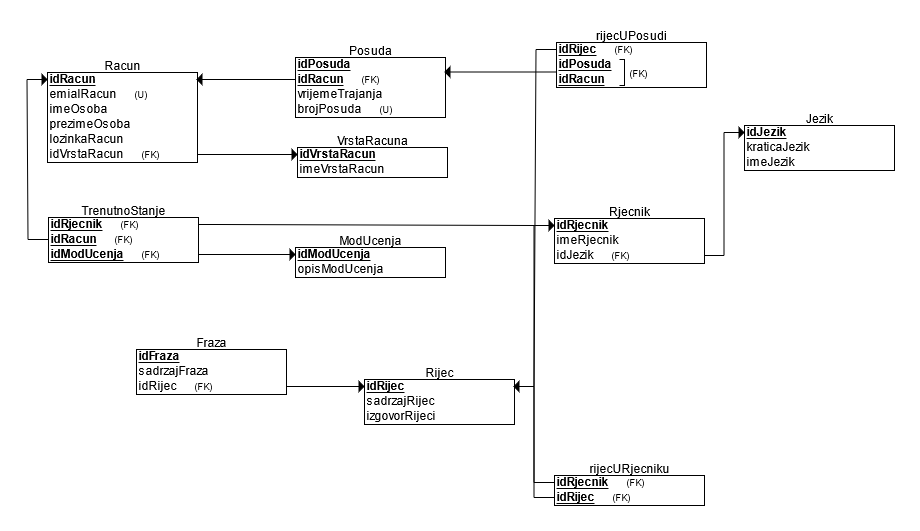
\includegraphics[width=\textwidth]{slike/dijagramBP.PNG}
					\caption{Dijagram baze podataka}
					\label{fig:dijagramBP}
				\end{figure}
				
				\newpage
			
			
		\section{Dijagram razreda}
		
			%\textit{Potrebno je priložiti dijagram razreda s pripadajućim opisom. Zbog preglednosti je moguće dijagram razlomiti na više njih, ali moraju biti grupirani prema sličnim razinama apstrakcije i srodnim funkcionalnostima.}\\
			
			%\textbf{\textit{dio 1. revizije}}\\
			
			%\textit{Prilikom prve predaje projekta, potrebno je priložiti potpuno razrađen dijagram razreda vezan uz \textbf{generičku funkcionalnost} sustava. Ostale funkcionalnosti trebaju biti idejno razrađene u dijagramu sa sljedećim komponentama: nazivi razreda, nazivi metoda i vrste pristupa metodama (npr. javni, zaštićeni), nazivi atributa razreda, veze i odnosi između razreda.}\\
			
			\begin{figure}[H]
				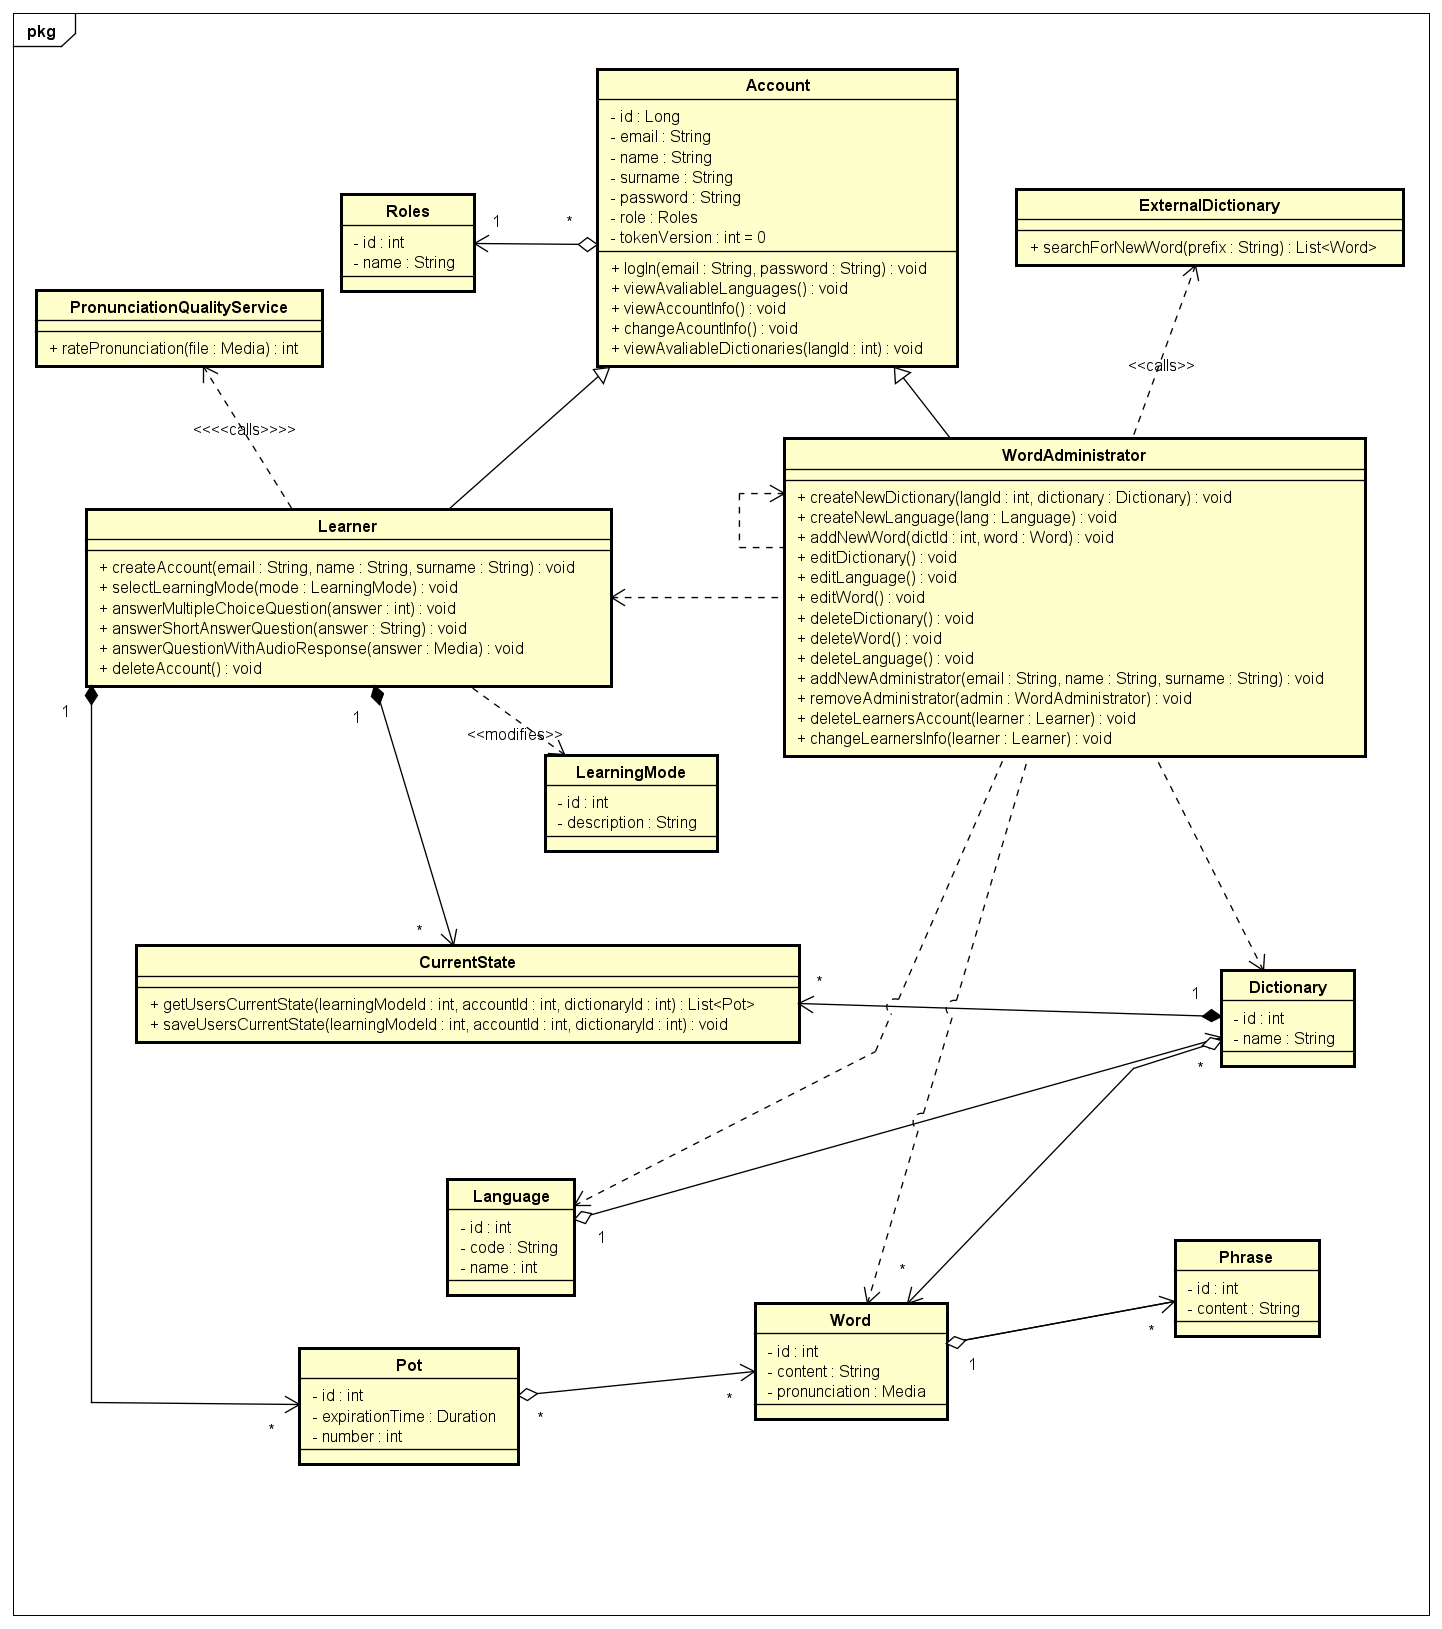
\includegraphics[width=\textwidth]{slike/ClassDiagram1.PNG}
				\caption{Dijagram razreda - modeli}
				\label{fig:classDiagram1}
			\end{figure}
			
			\newpage
			
			Slika 4.2 prikazuje razrede koji predstavljaju model u arhitekturi sustava. Dijagram je idejno razrađen. Čini ga razred Roles kojim označavamo o kojem se tipu korisničkog računa radi. On je vezan uz razred Account koji označava sam korisnički račun. Kako postoji više vrsta korisničkog računa te kako sve funkcionalnosti nisu iste za sve vrste korisničkih računa, postoje i razredi Learner i WordAdministrator koji su izvedene razreda Account razreda. Za razred WordAdministrator postoji rekurzivna ovisnost jer je moguće kreirati nove administratore riječi ako je korisnik također administrator riječi. Uz razred Learner veže se razred PronunciationQualityService koji je servis za ocjenu kvalitete izgovora riječi ako je učenik u tom modu učenja, razred LearningMode koji predstavlja mod učenja te ga učenik može promijeniti. Uz razred Learner također se veže i razred CurrentState koji označava trenutno stanje u kojem se učenik nalazi za prije odabrani rječnik. Nadalje, uz razred CurrentState veže se i razred Dictionary koji predstavlja rječnik. Uz rječnik je povezan razred Language jer rječnik pripada jeziku. Uz rječnik također je povezan i razred Word koji predstavlja riječ. Riječ je bolje opisana s nekoliko fraza koje su u modelu sustava razred Phrase. Uz razrede Learner i Word veže se i razred Pot koji je model posude u koju su spremljene riječi i to različito za svakog korisnika. Razredi Language, Word i Dictionary vezani su uz razred WordAdministrator jer administrator riječi može dodavati, brisati i mijenjati sadržaj jezika, rječnika i riječi. Na kraju, postoji i razred ExternalDictionary koji administrator riječi poziva ako želi dobiti prijedlog riječi koje zatim može dodati u neki od rječnika u sustavu. \newpage
			
			\begin{figure}[H]
				\includegraphics[width=\textwidth]{slike/ClassDiagram0.PNG}
				\caption{Dijagram razreda - generičke funkcionalnosti}
				\label{fig:classDiagram0}
			\end{figure}
			
			\newpage
			
			Slika 4.3 prikazuje detaljno razrađen dijagram razreda, ali samo za generičke funkcionalnosti sustava. Razred Account predstavlja istoimeni entitet u bazi podataka s brojnim metodama vezanima uz atribute entiteta, ali i uz autentifikaciju računa. On je povezan s enumeracijskim razredom Roles koji predstavlja listu svih mogućih vrsta korisničkog računa koji su korisnik, odnosno učenik, administrator riječi i korisnik koji se prvi put prijavljuje u sustav te tek mora promijeniti svoju zaporku kako bi mogao pristupiti svim funkcionalnostima sustava. Na dijagramu su također prikazana i dva bitna kontrolera. AuthenticationController provjerava i odgovara na zahtjeve za ulazak u sustav i izlazak iz istoga. AccountController služi za promjenu podataka u sustavu za korisnički račun te također služi i za uklanjanje računa iz sustava. Sučelje AccountService, razredi AccountServiceJpa kao njegova implementacija te AccountUserDetailsService služe za manipulaciju s korisničkim računima kroz bazu podataka. Slično, sučelje AuthenticationService i razred AuthenticationServiceJpa kao implementacija sučelja služe da ulazak u sustav te provjeru ispravnosti podataka kojima korisnik želi pristupiti sustavu. Razred AccountDTOMapper klasa je koja se nalazi na sloju \textit{Service} te služi za prijenos podataka o računu korisnika. Na sloju \textit{Repository} radnog okvira Spring nalazi se sučelje AccountRepository kojim je oblikovano dohvaćanje pohranjenih podataka u bazi podataka. Uz to, postoje i sigurnosni razredi koje služe za očuvanje sigurnosti podataka i sustava, a to su SecurityFilterChainConfig, SecurityController, SecurityConfig. Također, kako bi se vršila provjera ispravne autentifikacije te praćenje valjanosti sjednice, služe nam razredi JWTAuthenticationFilter te JWTUtil. Za početak rada aplikacije te unos početnih podataka u fazi razvoja postoji razred DataInitializer.
			
			\newpage
			
			\textbf{\textit{dio 2. revizije}}\\			
			
			\textit{Prilikom druge predaje projekta dijagram razreda i opisi moraju odgovarati stvarnom stanju implementacije}
			
			
			
			\eject
		
		\section{Dijagram stanja}
			
			
			%\textbf{\textit{dio 2. revizije}}\\
			
			%\textit{Potrebno je priložiti dijagram stanja i opisati ga. Dovoljan je jedan dijagram stanja koji prikazuje \textbf{značajan dio funkcionalnosti} sustava. Na primjer, stanja korisničkog sučelja i tijek korištenja neke ključne funkcionalnosti jesu značajan dio sustava, a registracija i prijava nisu. }
			
			\begin{figure}[H]
				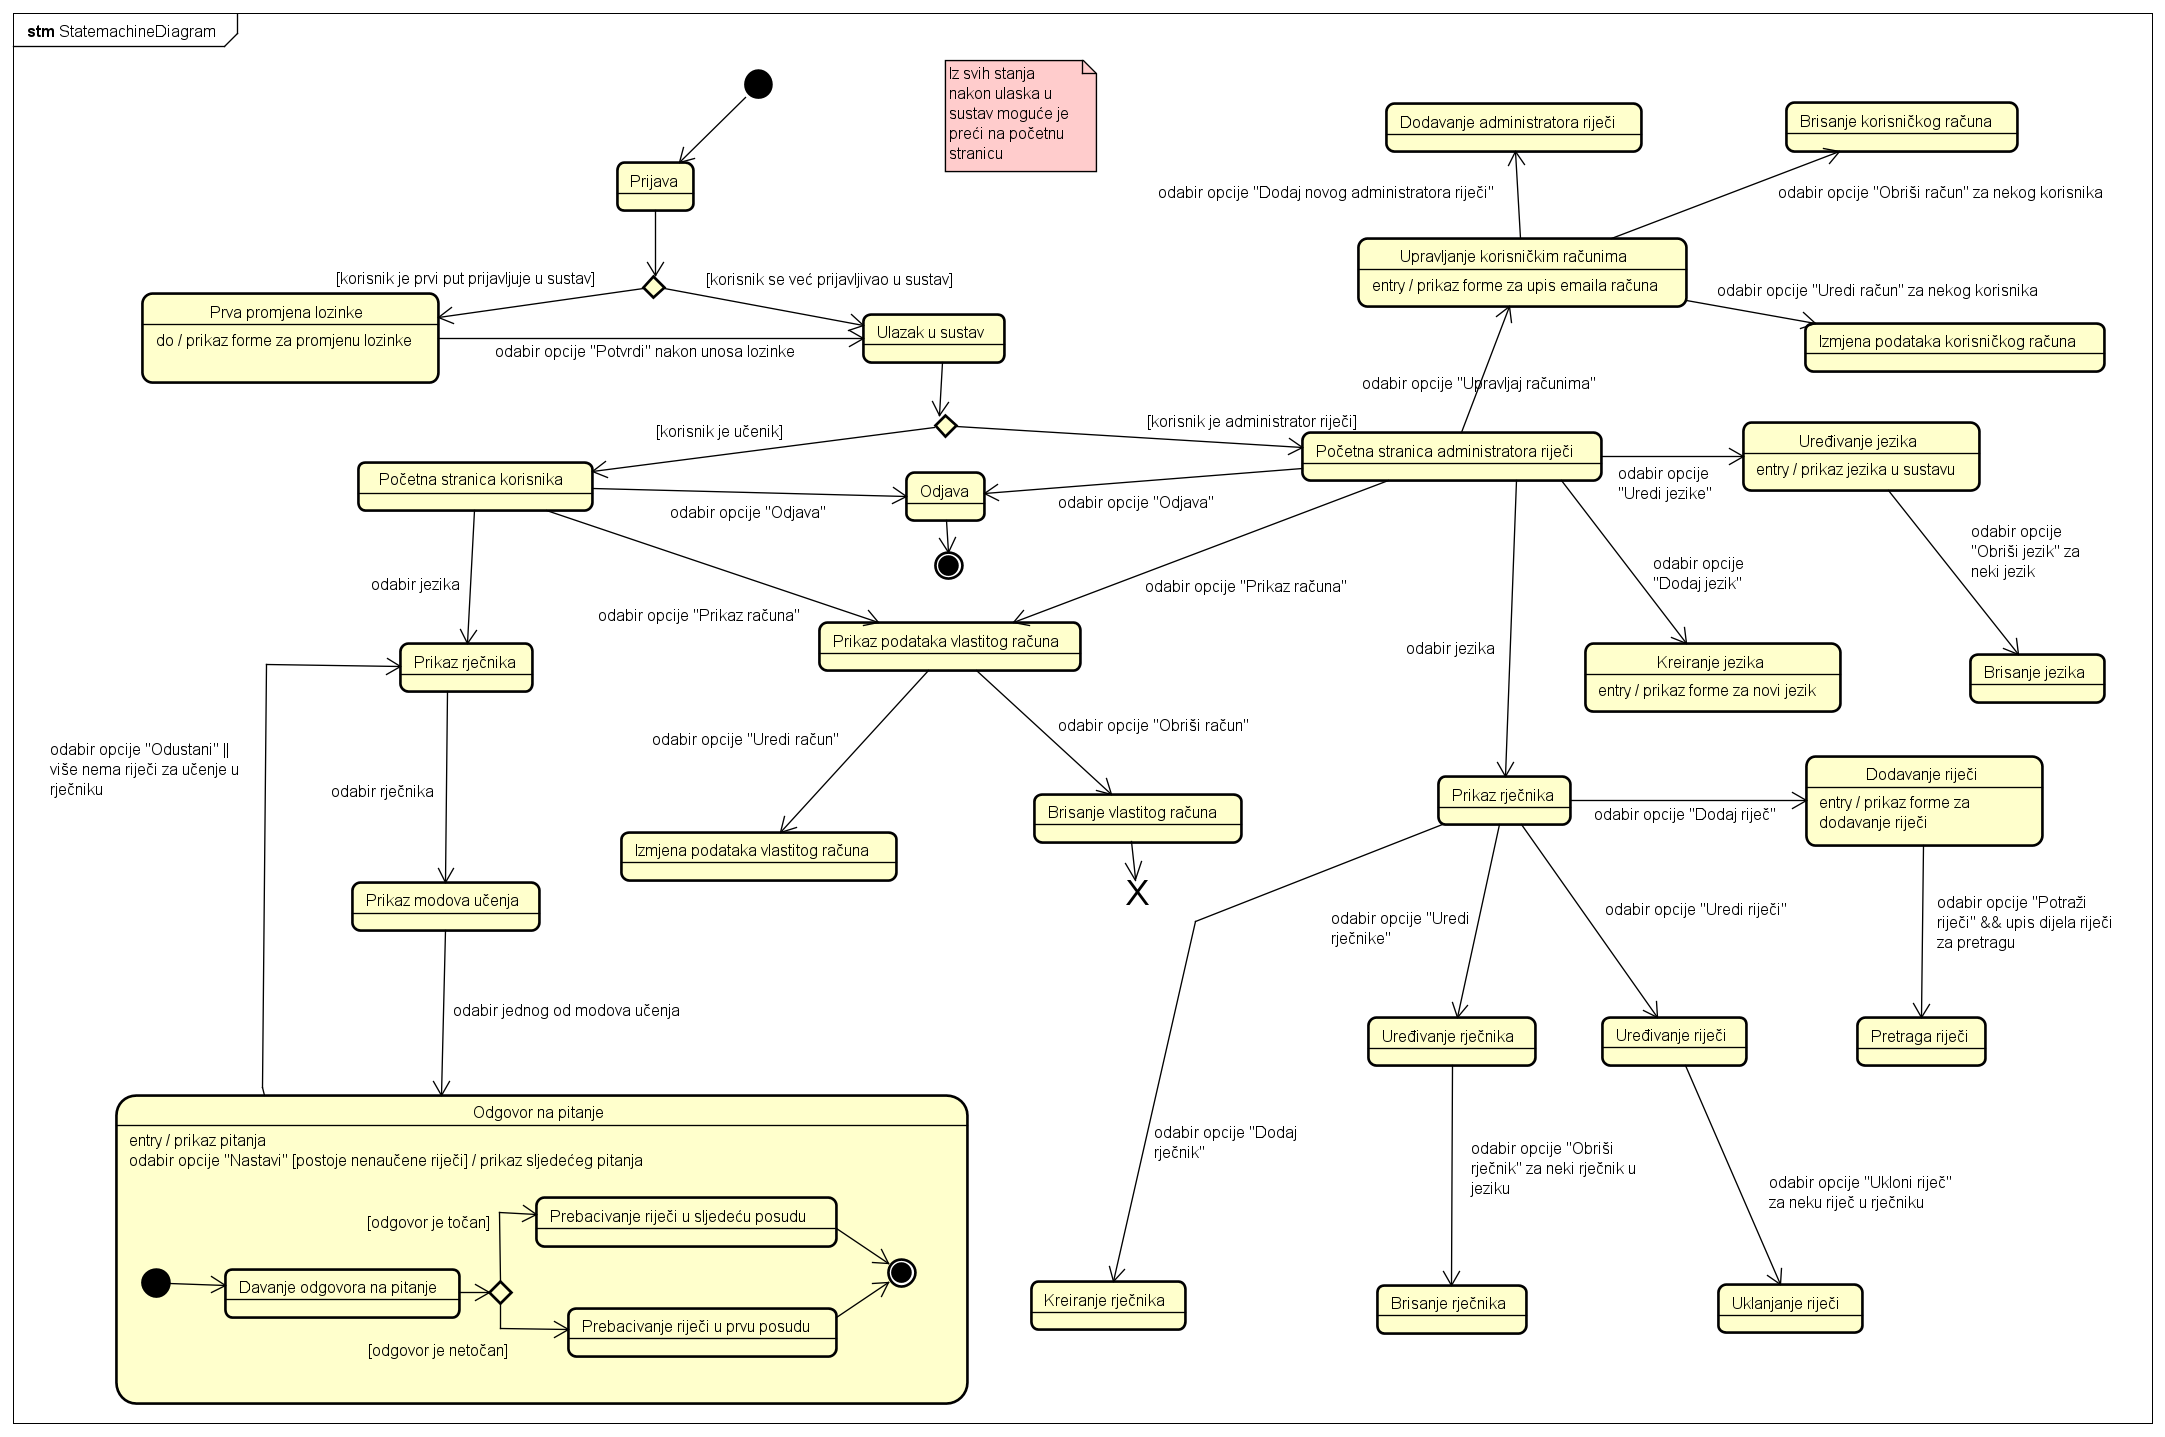
\includegraphics[width=\textwidth]{slike/StatemachineDiagram.PNG}
				\caption{Dijagram stanja - prikaz stanja sustava nakon prijave}
				\label{fig:statemachineDiagram}
			\end{figure}
			
			\newpage
			
			Slika 4.4 prikazuje dijagram stanja za velik dio sustava. Na dijagramu je prikazano u kojim se stanjima sustav može naći od trenutka prijave (ulaska u sustav) do odjave (napuštanja sustava) korisnika ovisno o tome koja je uloga korisnika, odnosno je li korisnik učenik ili administrator riječi. Prije samo ulaska u sustav, potrebno je provjeriti radi li se o korisniku koji se prvi put prijavljuje u sustav. Ako je to slučaj, tada se korisniku prikazuje stranica za prvu promjenu lozinke iz koje nije moguće izaći dok se ne upiše nova zaporka. Nakon uspješne promjene zaporke, korisnik kao i svi drugi pristupa sustavu u cijelosti. Ovisno o tome koje je vrste korisnički račun, korisniku se prikazuje početna stranica. Učenik s glavne stranice može otići na prikaz svojih podataka gdje iste može izmijeniti ili obrisati svoj račun, može se odjaviti ili može odabrati jedan od ponuđenih jezika. Odabirom jezika, sustav je u stanju prikaza rječnika korisniku. Ako korisnik odabere neki od rječnika, ulazi u stanje biranja jednog od modova učenja nakon čega se prikazuju pitanja. Pitanja se prikazuju dok to korisnik traži i dok postoje nenaučene riječi u posudama. Složeno stanje \textit{Odgovor na pitanje} prikazuje što sve sustav radi tijekom korisnikovog odgovaranja na pitanje. S druge strane, ako je korisnik administrator riječi, tada on kao i učenik može izmijeniti podatke vlastitog računa ili obrisati vlastiti račun ili odjaviti se iz sustava. Nadalje, administrator riječi može upravljati korisničkim računima. Ulaskom u stanje \textit{Upravljanje korisničkim računima} korisnik može birati između opcija dodavanja novog administratora riječi, izmjene nekog podatka za druge korisničke račune u sustavu ili može obrisati neki od korisničkih računa. Administrator riječi također može s početne stranice otići na kreiranje jezika, uređivanje jezike ili može odabrati neki od jezika na što se, slično kao i učeniku, otvara stranica s rječnicima za odabrani jezik. Ulaskom u \textit{Prikaz rječnika} administrator riječi može kreirati novi rječnik, urediti neki od postojećih rječnika, urediti neku od riječi u rječnicima i ukloniti rječnik ili riječ. Uz to, administrator riječi može odabirom opcije "Dodaj riječ" dodati novu riječ u sustav. Pri tome, može se poslužiti vanjskim rječnikom za lakše pronalaženje riječi koju želi dodati.
			
			\eject 
		
		\section{Dijagram aktivnosti}
			
			%\textbf{\textit{dio 2. revizije}}\\
			
			 %\textit{Potrebno je priložiti dijagram aktivnosti s pripadajućim opisom. Dijagram aktivnosti treba prikazivati značajan dio sustava.}
			
			\begin{figure}[H]
				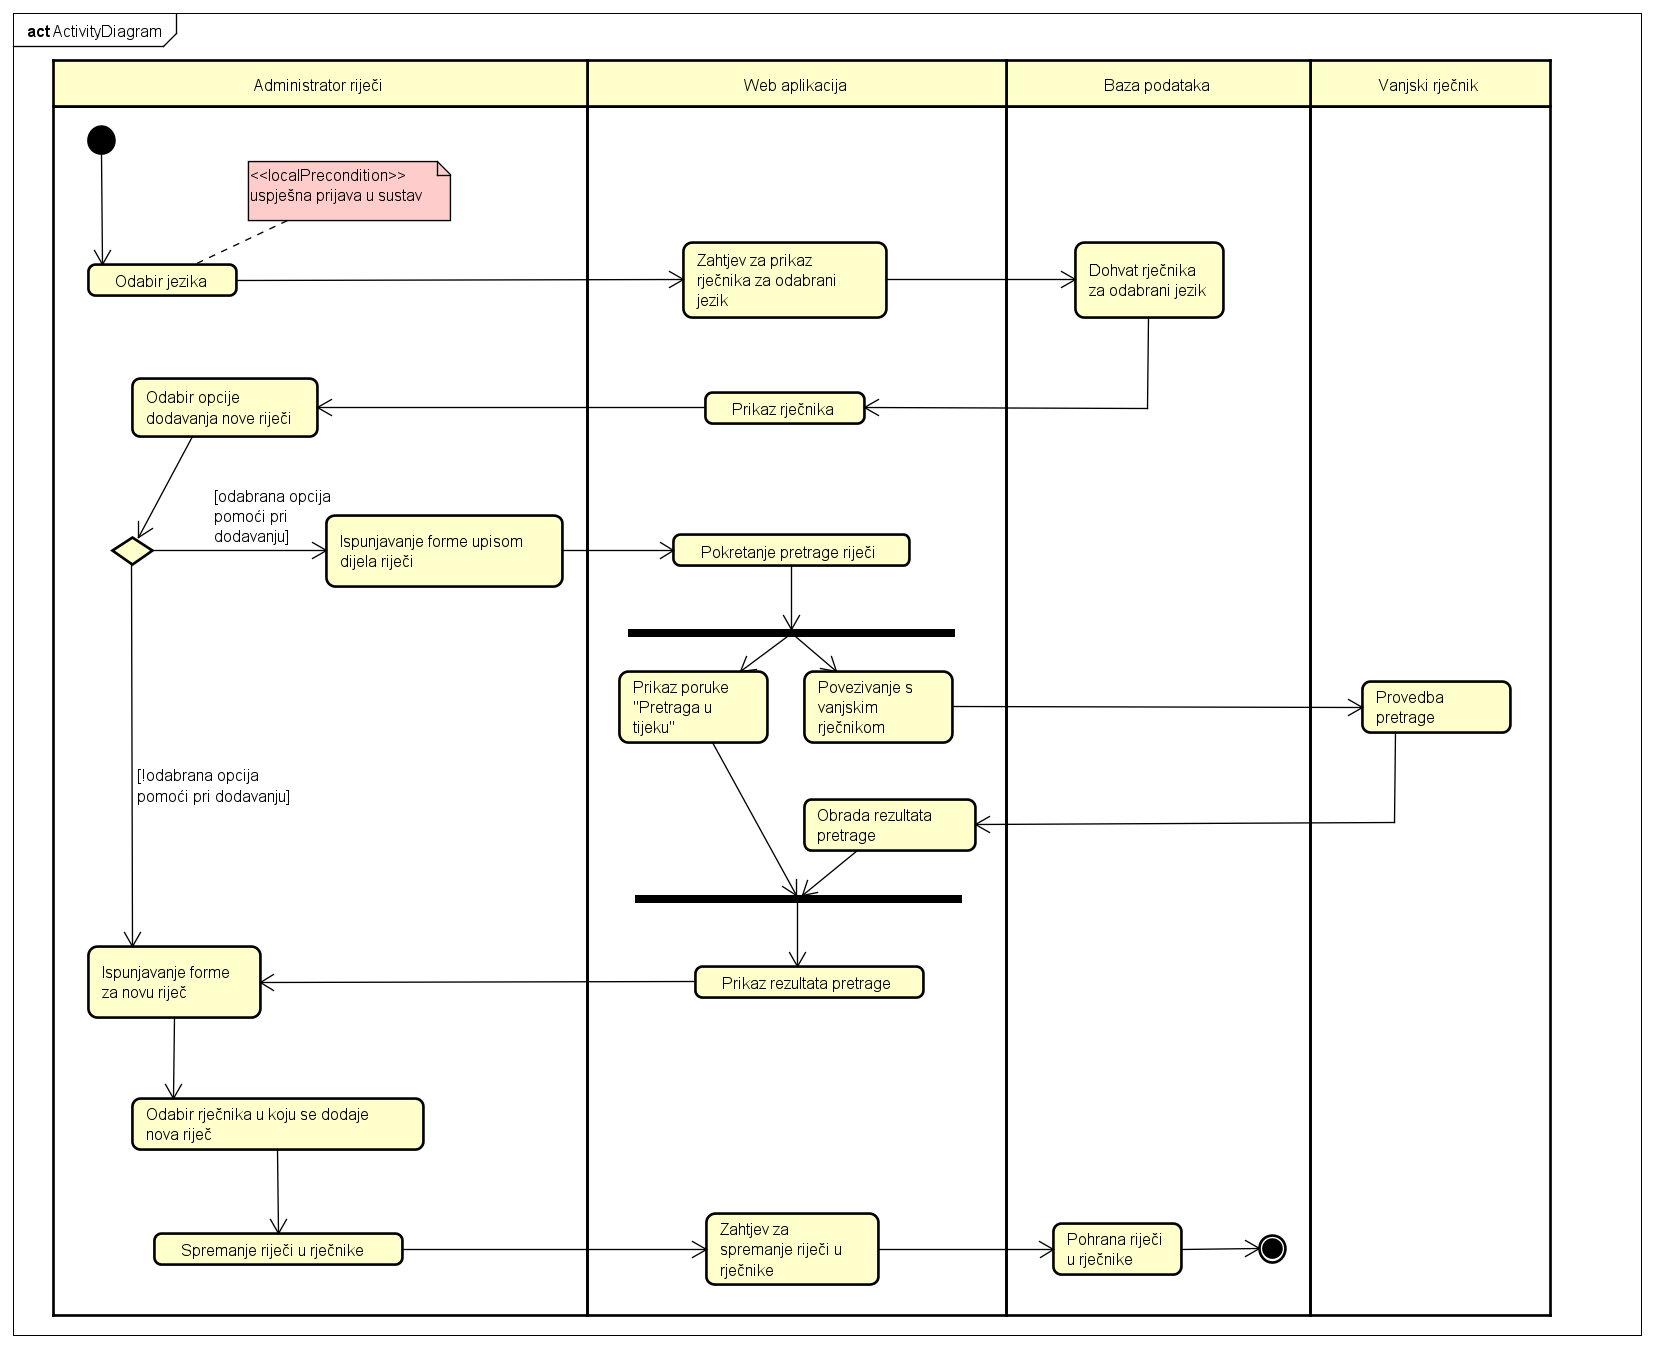
\includegraphics[width=\textwidth]{slike/ActivityDiagram.PNG}
				\caption{Dijagram aktivnosti - proces dodavanja nove riječi}
				\label{fig:activityDiagram}
			\end{figure}
			
			\newpage
			
			Slika 4.5 prikazuje dijagram aktivnosti. Na dijagramu je prikazan proces dodavanja nove riječi. Dijagram je podijeljen na particije koje odgovaraju aktorima koji sudjeluju u prikazanom procesu. Aktivnost započinje tako što administrator riječi odabire jezik. Uz to, nužan uvjet koji mora biti zadovoljen za odabir jezika je uspješna prijava u sustav, odnosno administrator riječi uspješno otvara početnu stranicu. Odabirom jezika, administrator riječi zapravo šalje zahtjev aplikaciji, a ona bazi podataka, za dohvat rječnika dostupnih za odabrani jezik. Nakon prikaza stranice sa svim rječnicima, administrator riječi odabire opciju dodavanja nove riječi. Pri dodavanju nove riječi, administrator riječi može potražiti pomoć od vanjskog rječnika upisom dijela riječi koju bi želio dodati te pokretanjem pretrage. Aplikacija pokreće pretragu riječi te dok traje spajanje aplikacije na vanjski servis administratoru riječi prikazuje poruku kako je pretraga u tijeku. uspješnim spajanjem aplikacije na vanjski rječnik i provedbom pretrage, aplikacija obrađuje rezultate pretrage te na koncu obavještava administratora riječi o rezultatima pretrage. Zatim, neovisno o tome je li administrator riječi odabrao opciju pomoći pri pretrazi, on ispunjava formu za novu riječ. Ispravnim popunjavanjem forme te odabirom rječnika, riječ se sprema u neki od rječnika čime završava aktivnost dodavanja riječi.
			
			\eject
		\section{Dijagram komponenti}
		
			%\textbf{\textit{dio 2. revizije}}\\
		
			 %\textit{Potrebno je priložiti dijagram komponenti s pripadajućim opisom. Dijagram komponenti treba prikazivati strukturu cijele aplikacije.}
			 
			 \begin{figure}[H]
			 	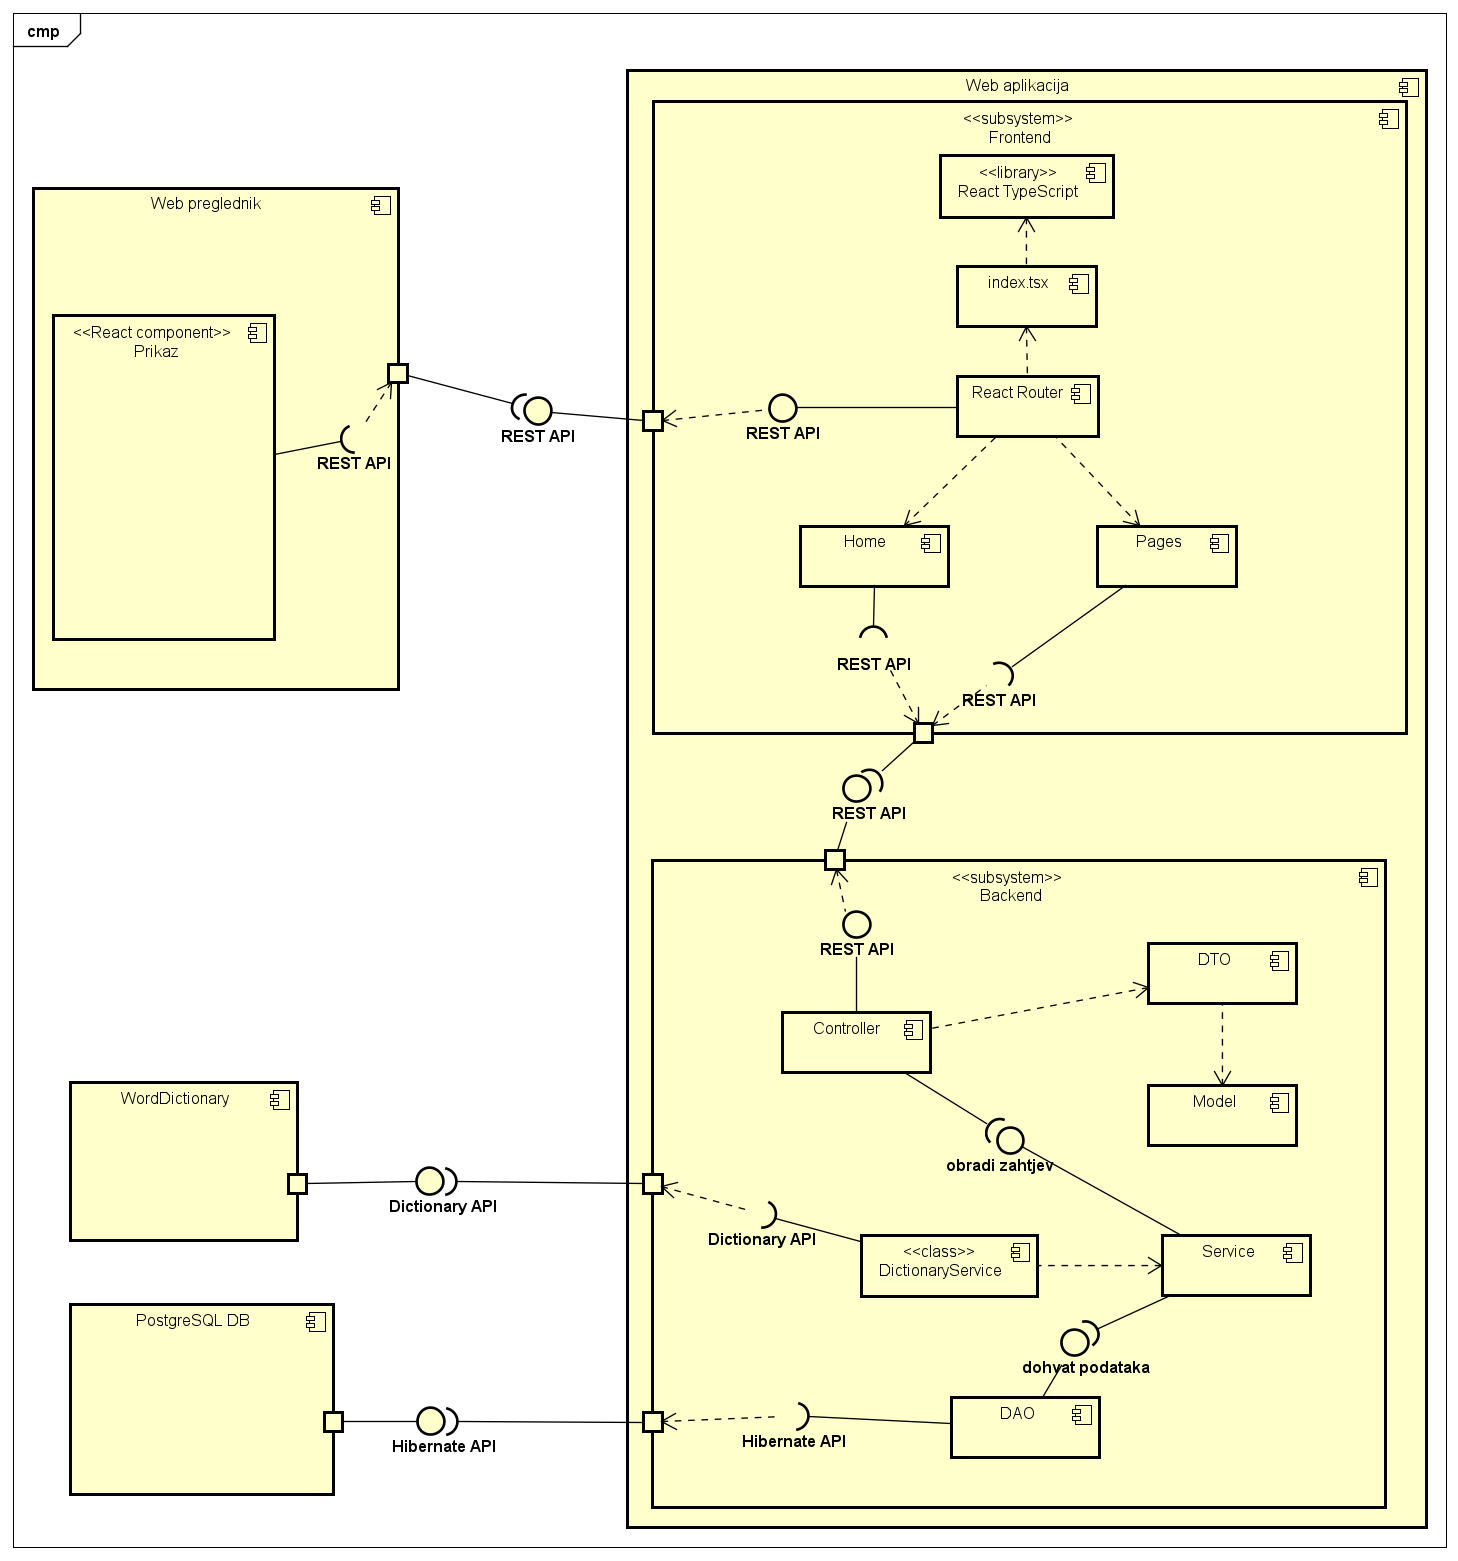
\includegraphics[width=\textwidth]{slike/ComponentDiagram.PNG}
			 	\caption{Dijagram komponenti}
			 	\label{fig:componentDiagram}
			 \end{figure}
			 
			 \newpage
			 
			 Slika 4.6 prikazuje dijagram komponenti. Dijagram komponenti prikazuje povezanost i organizaciju komponenti programske potpore. Glavne komponente od kojih se dijagram sastoji su Web preglednik, Web aplikacija, WordDictionary i baza podataka PostgreSQL. Sama Web aplikacija se sastoji od frontend i backend dijela. Klijent pristupa sustavu preko svog web preglednika. Web aplikacija, točnije frontend dio web aplikacija pruža sučelje koristeći REST API web pregledniku, a time i klijentu. Backend dio aplikacije komunicira s dvije komponente, komponentom WordDictionary i bazom podataka. Komponenta WordDictionary je vanjski rječnik preko kojeg web aplikacija pretražuje riječi koje se zatim mogu dodati u rječnike. Komunikacija između komponente WordDictionary i backend dijela web aplikacije ostvaruje se preko pripadnog Twinword API kojeg komponenta WordDictionary nudi web aplikaciji. Druga komponenta s kojom backend komunicira je PostgreSQL baza podataka. Baza podataka služi za pohranu svih podataka u sustavu. Komunikacije te dvije komponente ostvaruje se preko Hibernate API sučelja koje baza podataka nudi aplikaciji. Dijelovi web aplikacije ne rade neovisno, već postoji međusobna komunikacije te dvije komponente. Komunikacija se ostvaruje preko REST API-a. Frontend šalje backendu zahtjeve i podatke za obradu. Frontend dio sastoji se od glavne stranice i nekoliko rutera. Ruteri unutar aplikacije najopćenitije mogu se podijeliti na FirstLogIn koji se odnosi na stranicu koja se korisniku prikazuje prilikom prve prijave u sustav, Učenik i Administrator riječi koji služe za prikaz svih funkcionalnosti korisniku ovisno o tome kojeg je tipa korisnik. Svaki od rutera može komunicirati s backend dijelom aplikacije. S druge strane, backend dio od nešto više različitih komponenti. Backend dio aplikacije izgrađen je s pomoću Java Spring radnog okvira pa tako backend dio sadrži komponente poput Controller, Service, DAO. Komponenta Controller komunicira s frontend dijelom aplikacije te obradu dalje prosljeđuje kroz Service komponentu. Service komponenta sadrži poslovnu logiku aplikacije te može pristupati podacima iz baze podataka preko komponente DAO. DAO (Data Access Object) predstavlja Repository sloj u Spring aplikaciji i ona izravno može pristupati bazi podataka. Osim opisanih komponenti, backend dio aplikacije sadrži još neke komponente. DTO (Data Transfer Object) komponenta je koja služi za pretvorbu Modela u objekt. Model komponenta predstavlja sve entitete baze podataka. Osim ovih komponenti, dijagram komponenti sadrži i klasu DictionaryService koja je izdvojena iz komponente Service te predstavlja razred kojim se ostvaruje komunikacija s vanjskim rječnikom, odnosno komponentom WordDictionary.
			 